\subsection{Esiti delle verifiche dell'indice di Gulpease}
Di seguito è riportato il grafico dell'indice di Gulpease calcolato sui vari documenti, il cui valore è definito accettabile e ottimale come descritto nella sezione §2.2.1.1.\\
I dati fanno riferimento a:
\begin{itemize}
	\item \textbf{RR:} Revisione dei Requisiti;
	\item \textbf{RP:} Revisione di Progettazione (da aggiungere con l'avanzare del progetto);
	\item \textbf{RQ:} Revisione di Qualifica (da aggiungere con l'avanzare del progetto);
	\item \textbf{RA:} Revisione di Accettazione (da aggiungere con l'avanzare del progetto).
\end{itemize} 

\begin{figure}[H]
\centering
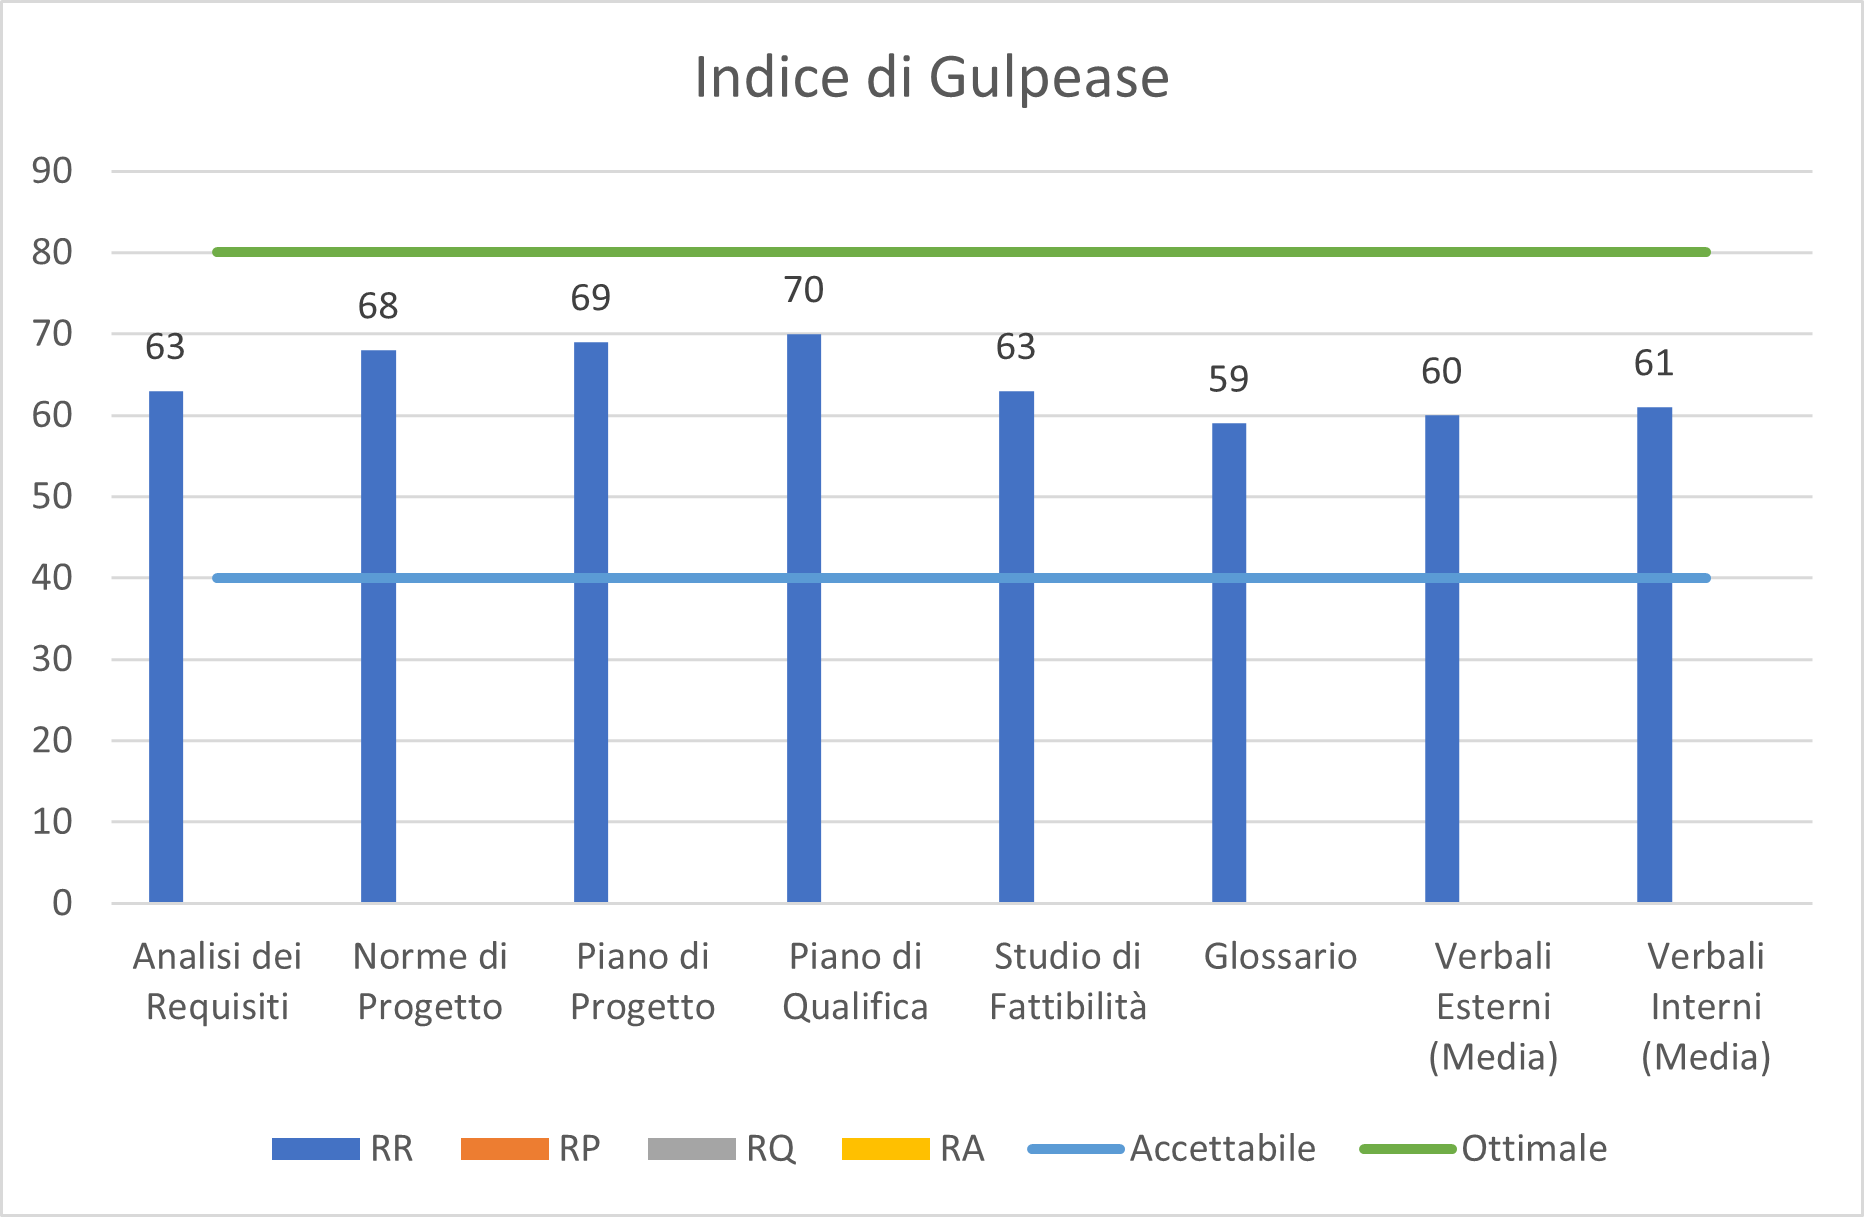
\includegraphics[scale=0.90]{res/ResocontoAttivitaDiVerifica/res/img/indiceGulpease.png}\\
\caption{Indice di Gulpease}
\end{figure}

